\section*{Results and Discussion}
To study the effects of multistability, non-linearities, boundaries and growth, we use a simple model which consists of a 2-node Turing topology system with non-linear Hill terms.
The activator A activates itself and I, while the inhibitor I inhibits the activator A.
However, instead of using the linear terms used in the original Turing system~\parencite{Turing1952}, we use Hill terms which represent genetic regulations.

\begin{subequations}
    \begin{equation}
        \pdv{[A]}{t}=b_{A}+V_{A} \cdot\frac{1}{1+\left(\frac{K{A}}{[A]}\right)^{n_{A}}}\cdot\frac{1}{1+\left(\frac{[I]}{K_{I}}\right)^{n_{I}}}-\mu_{A}\cdot[A] + D_{A}\nabla^2 [A]
    \end{equation}

    \begin{equation}
        \pdv{[I]}{t}=b_{I}+V_{I} \cdot\frac{1}{1+\left(\frac{K{A}}{[A]}\right)^{n_{A}}}-\mu_{I}\cdot[I] +
        D_{I}\nabla^2 [I]
    \end{equation}

    \label{eq:turinghill}
\end{subequations}
\subsection*{Multistability}
In this section, we demonstrate how linear stability analysis is not sufficient or necessary to predict Turing patterns (TPs) in multi-stable systems.
In particular, we study in detail the dynamical behaviour of multi-stable systems during pattern formation, which will lead to the creation or breaking of the pattern.
The motivation behind this arises from the high degree of multistability exhibited by biological systems, where cell-fate decisions have to be taken within this landscape ~\parencite{huang2000shape, moris2016transition}.
Multistability is especially common in systems with non-linearities and feedback loops, as the ones in biology or in our models~\parencite{pham2020complexity, leite2009multistability}.

Using the two-node non-linear Turing topology (Eq.~\ref{eq:turinghill}), multi-stable solutions were found and studied to understand how the patterning dynamics get affected when multiple steady-state solutions are found.
First, LSA is carried out on particular parameter sets to find multiple steady states with different stability nature (e.g.~stable, unstable, Turing I, Turing I-Hopf).
Then numerical simulations are computed where the initial condition is a random uniform distribution around a particular steady state.
Different pattern outcomes result depending on where in the phase diagram the initial condition is.
Following the classical hypothesis used in the Turing robustness literature, we would expect stable and unstable systems to not produce patterns and Turing to produce patterns.
Here, we present various examples of how this hypothesis can break under multistability conditions.

Fig.~\ref{fig:multistability1} shows a case where diffusion-driven instability conditions are not required for Turing pattern formation.
The unstable state, having a dispersion relation with a peak below zero (Fig.~\ref{fig:multistability1}C), managed to get into a Turing pattern regime as it is attracted by the neighbouring Turing steady state.
It therefore produces a stationary pattern (Fig.~\ref{fig:multistability1}B), even though its dispersion relation does not predict so.
This trajectory is depicted in the phase diagram (Fig.~\ref{fig:multistability1}A) which shows the steady states along with the vector field to understand the potential trajectories of the system.
The phase diagram does not fully capture the dynamics as it describes the system without diffusion, while the dispersion relation and the numerical solution do consider diffusion.

\begin{figure}[!h]
    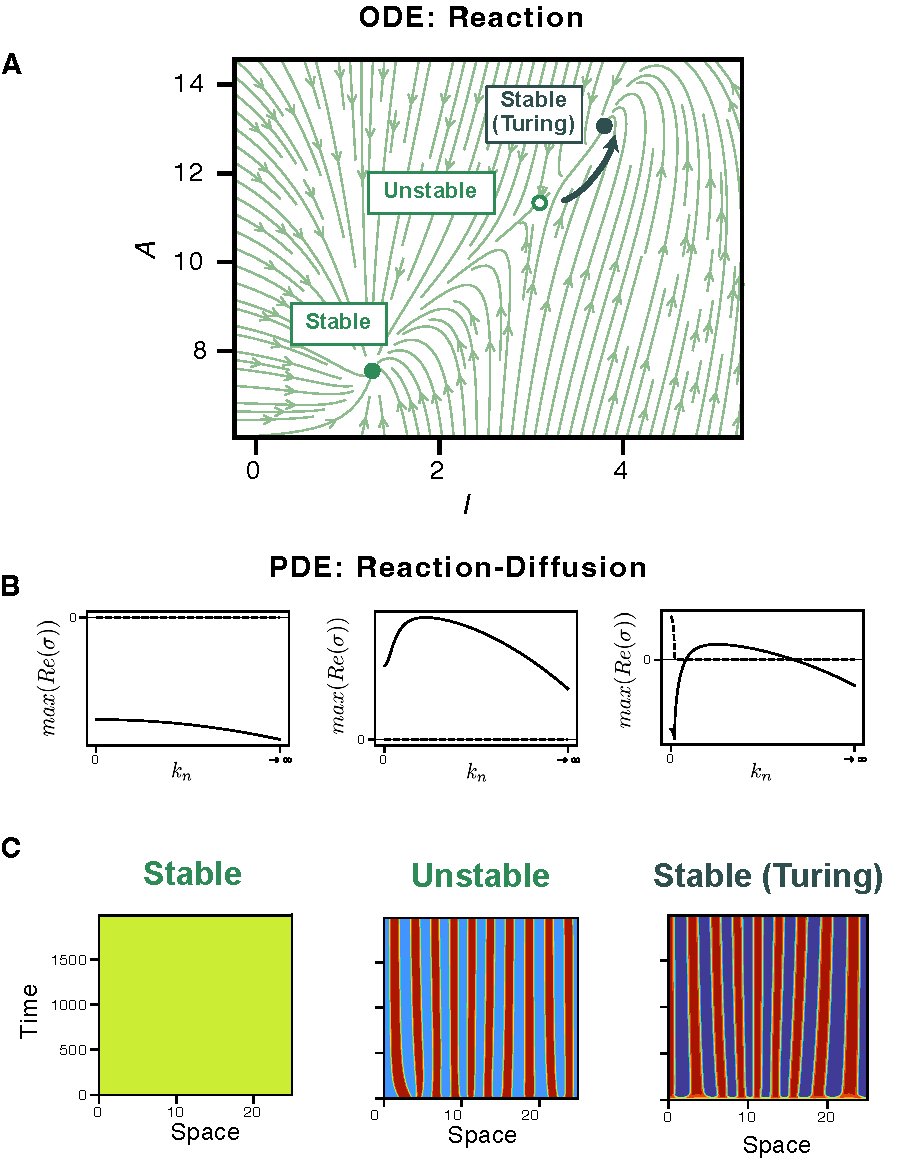
\includegraphics[width=1\textwidth]{figures/multistability1}

    \caption{\textbf{Stationary Patterns in multistability.} \textbf{(A)} Phase diagram without diffusion illustrating three distinct steady states where the derivative is zero: stable, unstable, and stable (Turing). These steady states are represented within a parameter space defined by two axes: concentrations of A and I. The vector field, indicated by light green arrows, shows the direction of the derivatives of the system at various points in the parameter space. A hand-drawn trajectory is also shown (dark green arrow), demonstrating how the unstable state may evolve into the Turing state. \textbf{(B)} Dispersion relation showing each type of state. \textbf{(C)} Numerical solutions of the three steady states with diffusion, where the unstable state unexpectedly produces a Turing-like stationary pattern. }
    \label{fig:multistability1} % A label for referencing this figure later in the document
\end{figure}



Then, we present a case where LSA incorrectly predicts stationary pattern formation.
Fig.~\ref{fig:multistability2} shows an ephemeral or transient pattern that occurs in the unstable and Turing regimes.
The TP initially develops in the vicinity of the Turing steady state.
As the spatial heterogeneity is amplified and settles, it gets attracted by the stable steady state leading to the disruption of the pattern.
This type of transient pattern behaviour has also been recently reported in~\cite{Krause2023}.

\begin{figure}[!h]
        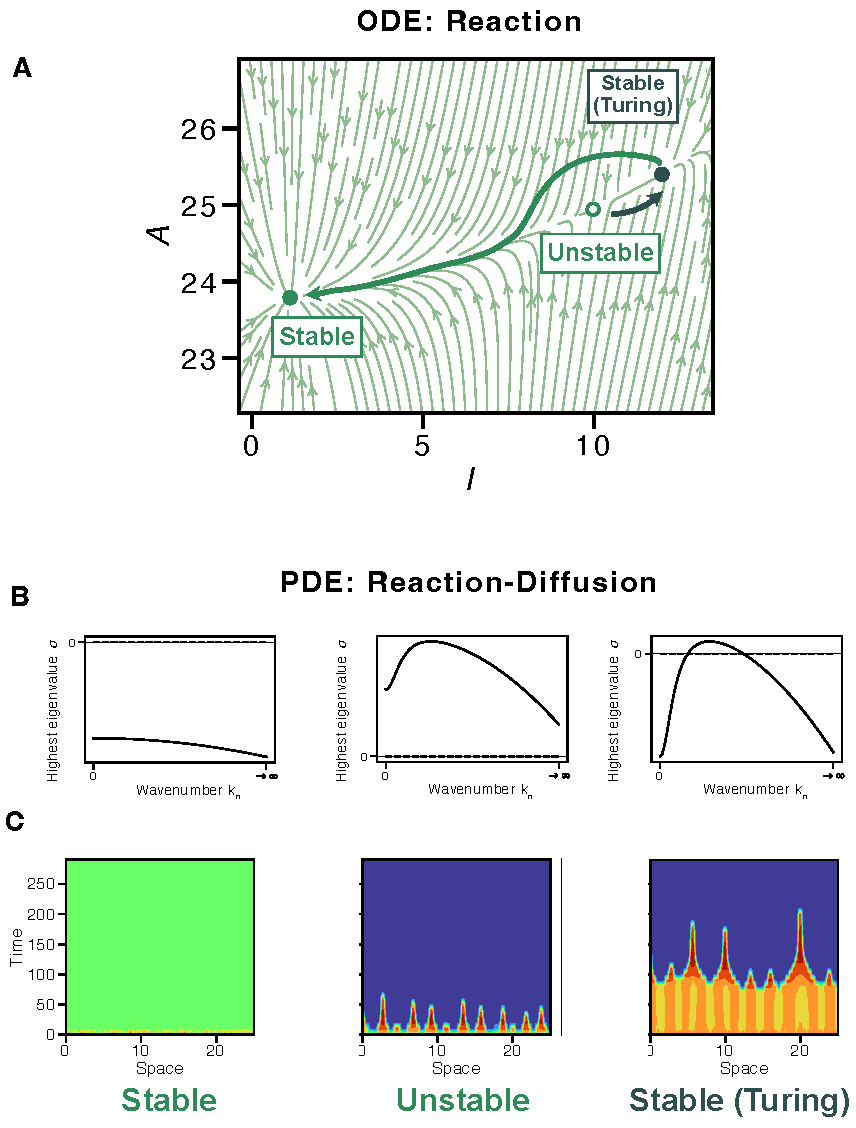
\includegraphics[width=1\textwidth]{figures/multistability2} % The name of your image file; assumes it is in the same directory as your .tex file
    \caption{\textbf{Ephemeral patterns in multistability.} \textbf{(A)} Phase diagram without diffusion illustrating three distinct steady states where the derivative is zero. The hand-drawn trajectory (dark green arrow) shows an unstable state evolving into a stable (Turing), and a stable (Turing) evolving into a stable. \textbf{(B)} Dispersion relation showing each type of state. \textbf{(C)} Numerical solutions of three steady states with diffusion. Unstable and Turing produce temporary periodic stationary patterns, that then disappear and become spatially homogeneous solutions.}
    \label{fig:multistability2} % A label for referencing this figure later in the document
\end{figure}

Other interesting examples can be found, for example, where an unstable state is surrounded by two Turing states, this unstable state will robustly lead to a Turing pattern (Fig.~\ref{sup_fig4}A).
Additionally, in some cases, the unstable system settles into Turing, but the Turing system gets pulled by the stable attractor (Fig.~\ref{sup_fig4}B). Additionally, some systems even exhibit three solutions which are homogeneous in time and space (Fig.~\ref{sup_fig4}C).
In this case, it would be worth investigating earlier time points with more resolution, as a pattern might appear then.
Interesting interactions similarly occur with multistability involving Turing I-Hopf solutions which will be mentioned in the following sections (Fig.~\ref{sup_fig4}D).

